We are now ready to perform the experiments. We will begin exploring SimCLR implementation and results, later we will explore BYOL's implementation and lastly we will compare them in order to see how BYOL tries to improve SimCLR and we will check if it is successful or not.

The code used for the experimentation, plus some files that contain the results, can be found on the Github repository made for this work.

\section{SimCLR exploration}
We will perform an iterative exploration with this framework. We will explore a few range for a subset of the hyperparameters and then we will go deeper into some hyperparameters to try to obtain better results.

\subsection{First approach}
\label{experiments:simclr:first}

The first thing we did to experiment with this framework is to explore a wide range of hyperparameters to see which set of them performed better for us. The script that can be found in \lstinline{code/SimCLR/run.py}.

What we did for this first exploration was to define a \emph{parameter grid} and execute the whole framework using each combination of the parameters. The parameters that were firstly considered are:
\begin{enumerate}
\item \lstinline{batch_size}. This is one of the most important parameters of SimCLR. In the original paper, it was proved that the higher this parameter, the better the results obtained for the linear classification. This parameter is also important since it has to adapt to our GPU's memory. The options that we have considered for the first experiments are: \lstinline|batch_size = {512,1024}|.

\item \lstinline{temperature}. The temperature parameter $\tau$ plays an important role in the individual loss seen in Equation \eqref{c:loss:simclr:ind}. It is suggested to try values in the range $[0,1]$ and the one that had better performance for the original experiments was around $0.5$, so we chose the following values: \lstinline|temperature = {0.25,0.5,0.75,1}|.

\item \lstinline{color_jitter_strength}. This parameter measures how hard is the color variation in the data augmentation. Previous results show that this parameter is important for the success of the network, so we provide with a big range of values. We include the following values: \lstinline|color_jitter_strength = {0.25,0.5,0.75,1}|.

\item \lstinline{epochs}. In the first stages of the experiments, we will always use $100$ as standard number of epoch for the trainings. We will see later if more epochs are needed in order to obtain better results.
\end{enumerate}

Using python and the python function \lstinline{itertools.product} we straightforwardly generate all possible different combinations of unions of the parameters so we only have to append them to a general string and execute the \lstinline{run.py} script mentioned before to obtain the results. In total, we obtain $32$ possible combinations, so we will obtain $32$ models. 

The script was executed and took approximately $24$ hours to train and evaluate all the different models, obtaining the results in Table \ref{table:simclr:gridsearch:1}.

\begin{table}[H]
    \centering
    
    \resizebox{\columnwidth}{!}{
    \begin{tabular}{rrrrrrr}
    batch\_size   & temperature   & color\_jitter & regularization\_loss & top\_1\_accuracy & top\_5\_accuracy & steps         \\ \hline
    \textbf{512}  & \textbf{0.25} & \textbf{0.25} & \textbf{0.0093}      & \textbf{0.833}          & \textbf{0.994}          & \textbf{9800} \\
                  &               & 0.5           & 0.0089               & 0.832                   & 0.993                   & 9800          \\
                  &               & 0.75          & 0.0086               & 0.831                   & 0.994                   & 9800          \\
                  &               & 1.0           & 0.008                & 0.83                    & 0.992                   & 9800          \\
                  & 0.5           & 0.25          & 0.0136               & 0.819                   & 0.993                   & 9800          \\
                  &               & 0.5           & 0.0124               & 0.822                   & 0.993                   & 9800          \\
                  &               & 0.75          & 0.0121               & 0.821                   & 0.993                   & 9800          \\
                  &               & 1.0           & 0.0118               & 0.817                   & 0.992                   & 9800          \\
                  & 0.75          & 0.25          & 0.0161               & 0.809                   & 0.993                   & 9800          \\
                  &               & 0.5           & 0.015                & 0.812                   & 0.993                   & 9800          \\
                  &               & 0.75          & 0.0141               & 0.805                   & 0.99                    & 9800          \\
                  &               & 1.0           & 0.0137               & 0.793                   & 0.99                    & 9800          \\
                  & 1.0           & 0.25          & 0.017                & 0.798                   & 0.99                    & 9800          \\
                  &               & 0.5           & 0.0163               & 0.797                   & 0.99                    & 9800          \\
                  &               & 0.75          & 0.016                & 0.793                   & 0.99                    & 9800          \\
                  &               & 1.0           & 0.0155               & 0.782                   & 0.989                   & 9800          \\
    \textbf{1024} & \textbf{0.25}          & 0.25          & 0.0103               & 0.836                   & 0.993                   & 4900          \\
                  &               & 0.5           & 0.0097               & 0.839                   & 0.995                   & 4900          \\
                  &               & \textbf{0.75} & \textbf{0.0093}      & \textbf{0.841}          & \textbf{0.995}          & \textbf{4900} \\
                  &               & 1.0           & 0.009                & 0.835                   & 0.993                   & 4900          \\
                  & 0.5           & 0.25          & 0.0149               & 0.822                   & 0.993                   & 4900          \\
                  &               & 0.5           & 0.0133               & 0.827                   & 0.994                   & 4900          \\
                  &               & 0.75          & 0.0132               & 0.826                   & 0.994                   & 4900          \\
                  &               & 1.0           & 0.0128               & 0.82                    & 0.993                   & 4900          \\
                  & 0.75          & 0.25          & 0.0168               & 0.814                   & 0.991                   & 4900          \\
                  &               & 0.5           & 0.0166               & 0.816                   & 0.992                   & 4900          \\
                  &               & 0.75          & 0.0157               & 0.813                   & 0.993                   & 4900          \\
                  &               & 1.0           & 0.0153               & 0.802                   & 0.989                   & 4900          \\
                  & 1.0           & 0.25          & 0.0175               & 0.806                   & 0.991                   & 4900          \\
                  &               & 0.5           & 0.0174               & 0.802                   & 0.992                   & 4900          \\
                  &               & 0.75          & 0.017                & 0.794                   & 0.99                    & 4900          \\
                  &               & 1.0           & 0.0164               & 0.79                    & 0.989                   & 4900         
    \end{tabular}
    }
    
    \caption{All results for first experiment using SimCLR using Resnet18.}
    
    \label{table:simclr:gridsearch:1}
    \end{table}

We have to remark, for each of the two possible batch sizes, the best results obtained. These are:

\begin{table}[H]
    \label{table:best:first:simclr}
\centering
\resizebox{\columnwidth}{!}{
\begin{tabular}{rrrrrrr}
batch\_size   & temperature   & color\_jitter & regularization\_loss & top\_1\_accuracy & top\_5\_accuracy & steps         \\ \hline
 512  &  0.25 &  0.25 &  0.0093      &  0.833         &  0.994          &  9800 \\
 1024 &    0.25       &  0.75 &  0.0093      &  \textbf{0.841}          &  0.995          &  4900 \\
\end{tabular}
}
\caption{Best results for the grid search experiment with SimCLR.}
\end{table}

\begin{remark}
On the original paper, the top 1 accuracy score reported for CIFAR10 in $100$ epochs was $\sim 84.6\%$ accuracy for batch size $512$ and $\sim 85.1 \%$ accuracy score for $1024$ batch size. It has to be remarked that these results were obtained using ResNet-50,  larger version of ResNet. It is also reported that larger encoder architectures benefit the model, so this is an advantage they have at this point of the experiments . Taking these aspects into account, and looking at the results obtained in our first experiment, we can say that this attempt was \emph{successful}.
\end{remark}

Let us make some observations. The clearest is that, since the second batch size doubles the first one, the training ends in half the steps. We can see that the temperature obtained in both cases is the same, and it is equal to $0.25$. However, there is a big change in the color jitter parameter: while using $512$ as batch size obtains the best result with the value of $0.25$ for color jitter, using $1024$ as batch size this value changes to $0.75$, which implies stronger color changes on the data augmentation. 

In general, having a look again at the Table \ref{table:simclr:gridsearch:1},  we can see that:

\begin{itemize}
    \item As it also happens in the experiments made on the original SimCLR paper, lower temperature $\tau$ parameters cause higher accuracies on the linear heads of our models.
    
    \item The models perform better when the \lstinline{color_jitter} parameter is in the range $[0.5,0.75]$. This means that, in general, a generous amount of color jittering to our picture is beneficial for the models.

    \item The \emph{Top 5 accuracy} is above $99\%$ in each model. This says that, since the models almost always give the correct label one of the 5 highest values, but they obtain the correct tag around $84\%$ of the times, they might be creating some similar representations of the data for inputs that do not belong to the same class. 
\end{itemize}

\subsection*{Observations about the batch size}

Although both models get to the same value of regularization loss, the model with a batch size of $1024$ obtains a higher \emph{top 1 accuracy}. This seems to follow the intuitive idea that we presented before: SimCLR benefits from bigger batch sizes since it allows a positive sample to be compared and pushed apart from negative samples. Ideally, we would keep pushing the batch size parameter forward, doubling it again to try to find out if the performance of the model keeps benefiting from bigger batch sizes. However, this requires either using multiple GPUs(or TPUs) working in parallel on the training or using GPUs with bigger memory, which we do not have access to. 

Using the resources we have, the following experiment was performed: using the hyperparameters that we found out in our \emph{GridSearch} to be the ones that achieve the best results except for the \lstinline{batch-size}, we train models moving the batch size in the following range: 
$$
\text{\lstinline{batch-size}}=\{16,32,64,128,256,512,1024\},
$$
where the last two values had already been computed in the GridSearch so we do not have to repeat the training. 

\begin{remark}
    To avoid confusion, we have to remark that in the figures that will come in the next pages, all the models do not end the training in the same number of steps because the number of steps depends on the \lstinline{batch_size}. That does not mean that the models were trained for a different number of epochs, and the figures are presented like this because Tensorboard provides the charts using the steps in the $x$ axis. 
\end{remark}

\begin{figure}[htp] 
    \centering
    \subfloat[Evolution of the top 1 accuracy with the batch size.]{%
        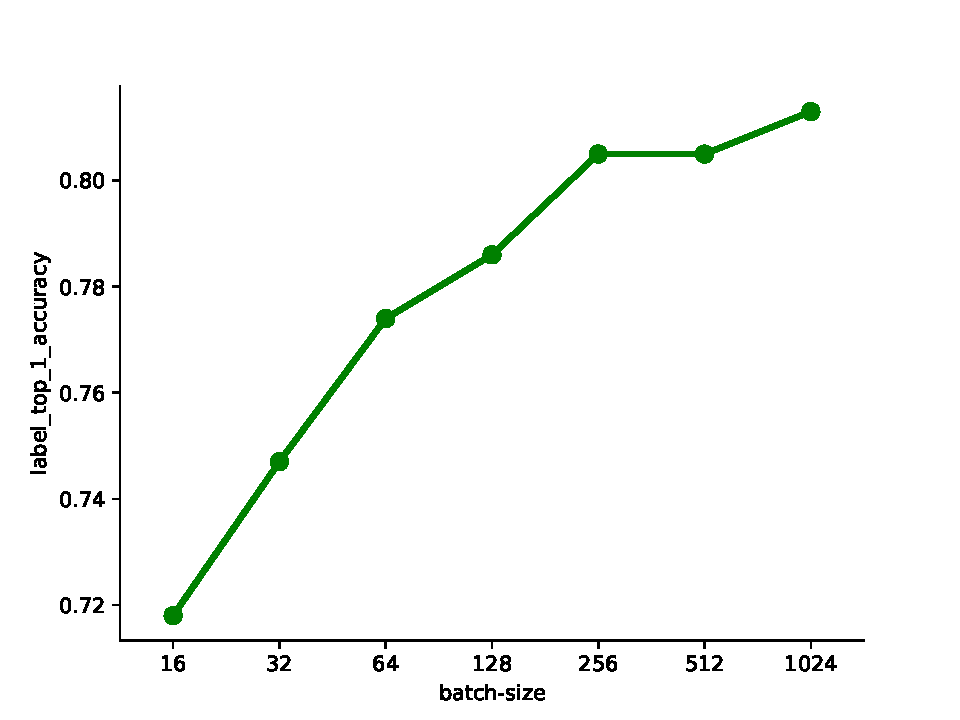
\includegraphics[width=0.45\textwidth]{simclr-batch-comparison}%
        \label{fig:accs:per:batch:simclr}%
        }%
    \hfill%
    \subfloat[Evolution curves of the accuracy with the steps taken in the training.]{%
        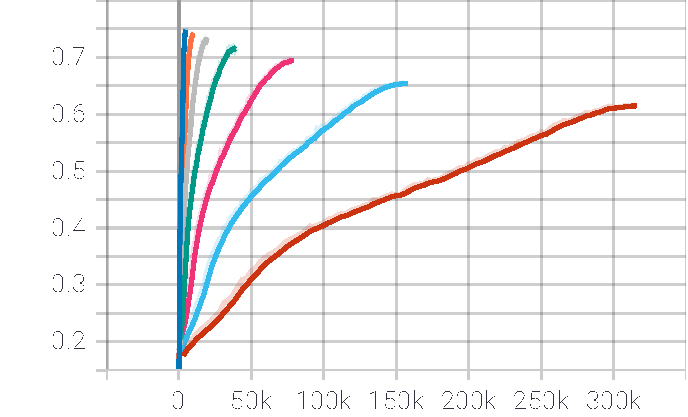
\includegraphics[width=0.45\textwidth]{train_supervised_acc}%
        \label{fig:evolution:acc:batches:simclr}%

        }%
        \caption{Results of the batch-size experiment.}
\end{figure}

Figure \ref{fig:accs:per:batch:simclr} shows the clear improvement of the Top 1 accuracy score when increasing the size of the batch that is used to compute the loss of our model. Increasing from $16$ to $1024$ gives an increase of more than $8\%$ in top 1 accuracy, which is a lot. Further increase can be obtained if we keep increasing the batch size, but this is beyond our computation possibilities.

Figure \ref{fig:evolution:acc:batches:simclr} supports what we have just presented: not only with a smaller batch size we have to do thousands of extra steps in the training, but also we obtain much better accuracy performance of the linear head of the model.

\subsection*{Observations of other hyperparameters}

We have seen that in our first experiment, batch size has been really relevant in the final results. We would like to see if the rest of the parameters play such an important role as well. 

As we have seen before, the parameters that we want to see how they affect the models are the \lstinline{color_jitter_strength} and the \lstinline{temperature} $\tau$ parameter. Let us study their impact on the model one by one. 

\begin{figure}[H] 
    \centering
    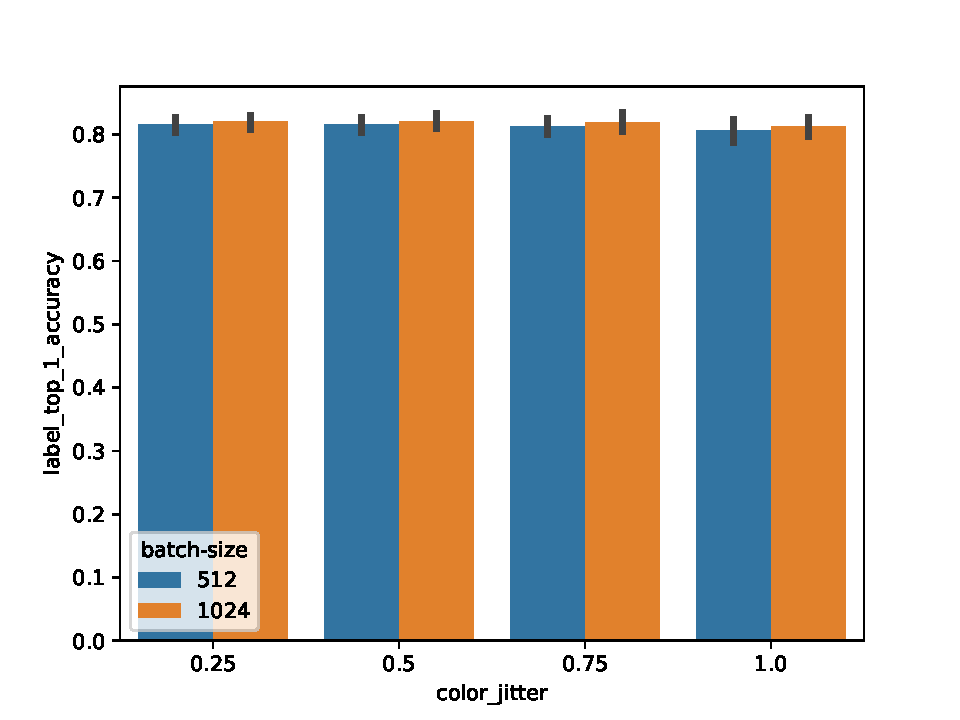
\includegraphics[width=0.55\textwidth]{color-jitter-impact-simclr}%
    
    \caption{Accuracy score following the color jitter parameter and both batch sizes considered.}
    
    \label{exp:simclr:colorjitter:impact}
\end{figure}

As we can see in Figure \ref{exp:simclr:colorjitter:impact}, the \lstinline{color_jitter_strength} parameter does not have a huge impact on the performance of the linear head of the model. The black bars on the center of each orange/blue bar indicate the variance of the accuracy respect the rest of the parameters. Surely, there are centesimal differences between the different values of this parameter. However, more finetuning might be needed in order to make this parameter relevant for our model. The low influence may as well be caused by the small encoder network (ResNet 18), so we will explore if there are any changes when we change the encoder network later in the document.

\begin{figure}[H] 
    \centering
        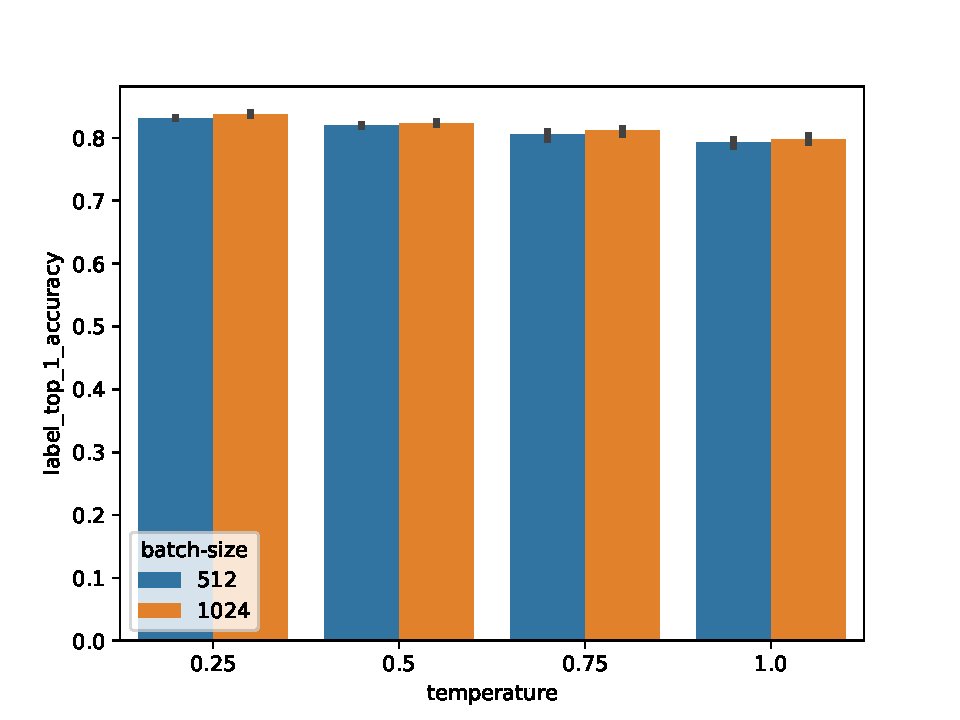
\includegraphics[width=0.55\textwidth]{temperature-impact-simclr}%
       
        \caption{Accuracy score following the temperature and both batch sizes considered.}
        
    \label{exp:simclr:temperature:impact}
\end{figure}

The parameter temperature, however, has a bigger impact on our framework's results. As we can see in Figure \ref{exp:simclr:temperature:impact}, when the temperature $\tau$ takes larger values, the accuracy obtained by the the linear head decreases. The decrease is approximately a $5\%$ on average, so we can affirm that the influence of the parameter is important on the model.

In the original paper, the best results also occurred with low values for the temperature parameter. They even tested lower values for this parameter and got even better results. We will take this into account for the following experiments.

\subsection{Going deeper on the encoder architecture}
\label{experiments:simclr:second}


As we have mentioned before, original results prove that using wider and deeper architectures for the encoder on the SimCLR framework. Going deeper, however, requires more computational capabilities since more parameters have to be adjusted.

In the implementation used, we have the option of changing an input parameter in order to execute the experiment with a different architecture for the encoder. Specifically, we can pass \lstinline{resnet_depth=50} as an argument to the \lstinline{run.py} script to execute the train of the framework and the linear head finetuning and evaluation with the Resnet50 architecture. The architecture for this neural network is presented in Table \ref{table:resnet:50}.


\begin{table}[H]
    \centering
    \begin{tabular}{|c|c|c|}
    \hline
    Layers                 & Output size                    & CIFAR10                         \\ \hline
    conv1                  & $112\times112$                 & $3\times3, \ 64,$ stride 1      \\ \hline
    \multirow{2}{*}{conv2} & \multirow{2}{*}{$56\times 56$} & $3\times3$ max pool, stride 2   \\ \cline{3-3} 
                           &                                & $\blockb{256}{64}{3}$           \\ \hline
    conv3                  & $28 \times 28$                 & $\blockb{512}{128}{4}$          \\ \hline
    conv4                  & $14 \times 14$                 & $\blockb{1024}{256}{6}$         \\ \hline
    conv5                  & $7 \times 7$                   & $\blockb{2048}{512}{3}$         \\ \hline
    \multirow{2}{*}{}      & $1\times 1$                    & $7\times 7$ global average pool \\ \cline{2-3} 
                           &                                & $10-d$ FC, softmax              \\ \hline
    \multicolumn{2}{|c|}{Number of parameters}              & $23.520.842$                    \\ \hline
    \end{tabular}
    \caption{Resnet50 architecture.}
    \label{table:resnet:50}
\end{table}

    As we can see comparing this architecture with ResNet18 in Table \ref{arch:resnet:18}, the number of parameters that the network has to train doubles the first one, so we expect to have less memory available on our GPU so the \lstinline{batch_size} will have to be decreased to be able to run the trainings. 
    
    This is clearly an issue, since we have already empirically shown  that our model benefits from taking larger values on this parameter. In this second stage of exploring the best parameters for SimCLR on CIFAR10, we used the following parameters set to perform our particular GridSearch:
    
    \begin{itemize}
        \item \lstinline{batch_size}. In this second experiment, due to the limitations in the GPU memory, we have to reduce the range of this parameter to:
        $$
        \text{\lstinline{batch-size}}=\{16,32,64,128,256\}.
        $$

        \item \lstinline{temperature}. We found out that, as it happens also to the original paper's experiments, lower temperature values help our representations to be better for downstream tasks. However, we decided to try again \emph{higher} temperature values again, that is: temperature values in the set $\{0.5,0.75\}$, to explore if the temperature parameter had any correlation with the encoder architecture.
        
        \item \lstinline{color_jitter_stregth}. This time we focus on harder (higher) color jitter strengths, testing in the range $\{0.65,0.75\}$, since in the first experiments the results obtained were better when this parameter was higher.
        
\end{itemize}

    Using this parameters, our script to train and evaluate the models using each combination was executed. The results obtained can be checked in Table \ref{table:simclr:gridsearch:2}.
    
    \begin{table}[H]
        \resizebox{\columnwidth}{!}{
        \begin{tabular}{rrrrrrr}
        batch\_size  & temperature  & color\_jitter & regularization\_loss & label\_top\_1\_accuracy & label\_top\_5\_accuracy & global\_step   \\ \hline
        32           & 0.5          & 0.65          & 0.0243               & 0.822                   & 0.992                   & 157762         \\
                     &              & 0.75          & 0.0238               & 0.814                   & 0.992                   & 157762         \\
        64           & 0.5          & 0.65          & 0.0223               & 0.835                   & 0.995                   & 78881          \\
                     &              & 0.75          & 0.0222               & 0.833                   & 0.994                   & 78881          \\
                     & 0.75         & 0.25          & 0.021                & 0.838                   & 0.995                   & 78881          \\
                     &              & 0.65          & 0.0242               & 0.828                   & 0.993                   & 78881          \\
                     &              & 0.75          & 0.0243               & 0.822                   & 0.993                   & 78881          \\
        128          & 0.5          & 0.65          & 0.0225               & 0.844                   & 0.994                   & 39100          \\
                     &              & 0.75          & 0.0222               & 0.842                   & 0.994                   & 39100          \\
                     & 0.75         & 0.65          & 0.0248               & 0.831                   & 0.994                   & 39100          \\
                     &              & 0.75          & 0.024                & 0.829                   & 0.994                   & 39100          \\
        \textbf{256} & \textbf{0.5} & 0.65          & 0.0235               & 0.846                   & 0.995                   & 19695          \\
                     &              & \textbf{0.75} & \textbf{0.023}       & \textbf{0.848}          & \textbf{0.994}          & \textbf{19695} \\
                     & 0.75         & 0.65          & 0.0255               & 0.832                   & 0.994                   & 19695          \\
                     &              & 0.75          & 0.0262               & 0.833                   & 0.994                   & 19695         
        \end{tabular}
        }
    
        \caption{All results for the SimCLR first experiment using Resnet50}
        \label{table:simclr:gridsearch:2}    
    \end{table}
    
    We remark in Table \ref{table:best:second:simclr} some of the most interesting results, comparing them with the ones obtained in the first experiment.

    \begin{table}[H]
    \centering
    \resizebox{\columnwidth}{!}{
    \begin{tabular}{rlllllll}
    resnet\_depth & batch\_size   & temperature   & color\_jitter & regularization\_loss & top\_1\_accuracy & top\_5\_accuracy & steps         \\ \hline
    18 & 512  &  0.25 &  0.25 &  0.0093      &  0.833         &  0.994          &  9800 \\
     & 1024 &    0.25       &  0.75 &  0.0093      &  0.841          &  0.995          &  4900 \\
    \textbf{50} & 128 & 0.5 & 0.65 & 0.0225 & 0.844 & 0.994 & 39100 \\
     & \textbf{256} & \textbf{0.5} & \textbf{0.75} & \textbf{0.023} & \textbf{0.848} & \textbf{0.994} & \textbf{19695} 
    \end{tabular}
    }
    \caption{Best results for the second grid search experiment with SimCLR.}
    
    \label{table:best:second:simclr}
    \end{table}

    As we can see, the results of the models that use ResNet50  as an encoder outperform the ones that use ResNet18 for a few hundredths in the top 1 accuracy score, and also they reach a lower value in the loss function. Since it is clear that the gain we obtain by increasing the encoder depth is minimal, we may think that it is not worth it for our model since the number of parameters that have to be trained and, thus, the time that the train takes is much higher. However, we must not forget a very important fact that we observed in the first experiment: SimCLR benefits from bigger batch sizes. The results are comparing batch sizes $512$ and $1024$ in the first experiment with $128$ and $256$ in the second experiment (as we have already mentioned, the GPU memory does not allow us to use a bigger batch size when we increase the encoder depth).

    Taking this into account and although we can not empirically prove it, we state that when the batch size is increased as well as the encoder depth, the models with larger depth will outperform the models using ResNet18. Let us see some more details about the training.

    In the official implementation of SimCLR, two losses are computed: a contrastive loss and a supervised loss. The total loss is computed as the sum of both:
    \[
    \mathcal L_{\operatorname{total}} = \mathcal L_{\operatorname{contrastive} }+ \mathcal L_{\operatorname{supervised}}.    
    \]

\begin{remark}
The figures that will be shown during this chapter show charts of the evolution of certain values. The plots have been smoothed automatically by Tensorboard, using the default smoothing parameter: $0,6$. Some \emph{shadows} may appear in the charts, corresponding to the original values that the curve took before it was smoothed.
\end{remark}

    We can visualize how the loss evolve through the training using the Tensorboard output. The lines are smoothed, that is why sometimes there might be some \emph{shadows} near the lines. The smoothing coefficient is set as default ot $0,6$. 
    \begin{figure}[htp] 
        \centering
        \subfloat[Contrastive loss in train]{%
            \includegraphics[width=0.45\textwidth]{simclr-exp2/train_contrast_loss}%
            \label{fig:contrastive:loss:exp2}%
            }%
        \hfill%
        \subfloat[Supervised loss in train]{%
            \includegraphics[width=0.45\textwidth]{simclr-exp2/train_supervised_loss}%
            \label{fig:supervised:loss:exp2}%
    
            }%
            \caption{Charts of the losses during train in second experiment. On axis $x$ we have the number of steps and on $y$ axis the value of the loss.}
            \label{fig:exp2:both:losses}
    \end{figure}


\begin{figure}[H]
\centering
\includegraphics[width=0.55\textwidth]{simclr-exp2/train_total_loss}%
\caption{Total loss of the four remarked models in the second experiment. The axis are the same of the ones in Figure \ref{fig:exp2:both:losses}. }
\label{fig:total:loss:exp2}%
\end{figure}

As we can see, although the loss is a sum of two components, as the steps/epochs get close to the end of the training, the supervised loss tends to zero. However, the contrastive loss remains in the range $[8,9.5]$ approximately. 

If we have a look at Figure \ref{fig:supervised:loss:exp2} we can see that in all cases it reaches a minimum and although more steps of the experiments are done, the value of this loss does not get reduced. However, if we have a look at the contrastive loss in Figure \ref{fig:contrastive:loss:exp2}, we can see that in three out of the four models, the loss is still decreasing and if we increased the number of epochs,we state that we would probably obtain better results.

\subsection{Gaussian blur in the image augmentations}
\label{exp3:adding:blur}

We have also studied if adding \emph{gaussian blur} as a part of the data augmentation process. This can be easily done by adding to the execution command the parameter \lstinline{--use_blur=True} to the run script. As we have already mentioned, the types of transformations applied in the data augmentation process is very relevant for the model training. The quality of the representations strongly depends on the transformations used.

Our goal with adding gaussian blur to the experiment is testing if, in the case of this specific dataset (CIFAR10), adding gaussian blur as a part of the data augmentation improves the quality of the representations for the classification task performed later. It is very important to remark that we are testing this \emph{only} for this dataset. The results obtained for this dataset do not have to be verified in general, since we know that most of the times, training a model in a dataset involves searching for the best hyperparameters for the specific dataset.

For this experiments, we decided to use wide range of hyperparameters and perform a third \emph{grid search}. Concretely, we chose:
\begin{itemize}
\item \lstinline{resnet_depth}. Although we already know and have proved that SimCLR benefits from larger ResNet depths, we wanted to see if adding data augmentation to the pretrain phase also improves the results of the smaller ResNet depths. Because of this, we trained models on both \emph{ResNet18} and \emph{ResNet50}.
\item \lstinline{batch_size}. In this case, we fix a batch size of $256$ for the ResNet50 trainings, since we already know that we can not fit bigger batch sizes in the GPU's memory. For the ResNet18 models, we test the same size that we use in ResNet50, and also add two bigger values to see how the model performs, so we use the set $\{256,512,1024\}$.
\item \lstinline{temperature}. In previous cases, the value that performed the best for us was $0.25$. However, since in the original paper suggest to use $0.5$ since it is the best parameter for \emph{ImageNet}, we use this value as well, obtaining the set $\{0.25,0.5\}$.
\item \lstinline{color_jitter_strength}. We use again the values $\{0.65,0.75\}$ since we obtained before good results using these two values.
\end{itemize}

Using these parameters, we obtain the results that we depict in Table \ref{table:simclr:gridsearch:blur}. 
\begin{table}[H]
    \resizebox{\columnwidth}{!}{
    \begin{tabular}{rrrrrrrr}
    resnet\_depth & batch\_size  & temperature   & color\_jitter & regularization\_loss & label\_top\_1\_accuracy & label\_top\_5\_accuracy & global\_step   \\ \hline
    18            & 256          & 0.25          & 0.65          & 0.0072               & 0.827                   & 0.992                   & 19695          \\
                  &              &               & 0.75          & 0.007                & 0.825                   & 0.994                   &                \\
                  &              & 0.5           & 0.65          & 0.0108               & 0.819                   & 0.993                   &                \\
                  &              &               & 0.75          & 0.0108               & 0.82                    & 0.993                   &                \\
                  & 512          & 0.25          & 0.65          & 0.0081               & 0.841                   & 0.993                   & 9800           \\
                  &              &               & 0.75          & 0.0081               & 0.837                   & 0.994                   &                \\
                  &              & 0.5           & 0.65          & 0.012                & 0.824                   & 0.994                   &                \\
                  &              &               & 0.75          & 0.0118               & 0.823                   & 0.994                   &                \\
                  & 1024         & 0.25          & 0.65          & 0.0093               & 0.846                   & 0.994                   & 4900           \\
                  &              &               & 0.75          & 0.0092               & 0.841                   & 0.995                   &                \\
                  &              & 0.5           & 0.65          & 0.0132               & 0.83                    & 0.994                   &                \\
                  &              &               & 0.75          & 0.0131               & 0.833                   & 0.994                   &                \\
    \textbf{50}   & \textbf{256} & \textbf{0.25} & \textbf{0.65} & \textbf{0.0228}      & \textbf{0.862}          & \textbf{0.997}          & \textbf{19695} \\
                  &              &               & 0.75          & 0.0224               & 0.861                   & 0.996                   &                \\
                  &              & 0.5           & 0.65          & 0.0223               & 0.849                   & 0.996                   &                \\
                  &              &               & 0.75          & 0.0215               & 0.851                   & 0.995                   &               
    \end{tabular}
    }
    \caption{Results for SimCLR using the best hyperparameters found in previous experiments, plus adding the Gaussian Blur to training preprocessing.}
    \label{table:simclr:gridsearch:blur}
    \end{table}


The models that obtained the best results in terms of Top 1 Accuracy are the following:

\begin{table}[H]
    \resizebox{\columnwidth}{!}{
    \begin{tabular}{rrrrrrrr}
    resnet\_depth & batch\_size  & temperature   & color\_jitter & regularization\_loss & label\_top\_1\_accuracy & label\_top\_5\_accuracy & global\_step   \\ \hline

    18              & 1024         & 0.25          & 0.65          & 0.0093               & 0.846                   & 0.994   &  4900                     \\
    \textbf{50}   & \textbf{256} & \textbf{0.25} & \textbf{0.65} & \textbf{0.0228}      & \textbf{0.862}          & \textbf{0.997} & \textbf{19695}          \\                                
    \end{tabular}
    }
    \caption{Best results for the experiment of adding gaussian blur to data augmentation.}
    \label{table:simclr:gridsearch:blur:best}
\end{table}

As we can see, the model that uses ResNet50 outperforms the one using a smaller ResNet architecture, as expected. Also, the temperature parameter obtained the best results before, does it again in in this experiment, obtaining a final Top 1 accuracy of $0.862$.




    \begin{table}[H]
        \resizebox{\columnwidth}{!}{
        \begin{tabular}{lrrrrrrrr}
        Experiment &resnet\_depth & batch\_size  & temperature   & color\_jitter & regularization\_loss & label\_top\_1\_accuracy & label\_top\_5\_accuracy & global\_step   \\ \hline 
    1st& 18 & 1024 &    0.25       &  0.75 &  0.0093      &  0.841          &  0.995          &  4900 \\
    2nd& 50 & {256} & {0.5} & {0.75} & {0.023} & {0.848} & {994} & {19695}  \\
    \textbf{3rd}&    18              & 1024         & 0.25          & 0.65          & 0.0093               & 0.846                   & 0.994   &  4900                     \\
    & \textbf{50}   & \textbf{256} & \textbf{0.25} & \textbf{0.65} & \textbf{0.0228}      & \textbf{0.862}          & \textbf{0.997} & \textbf{19695}                                                     
        \end{tabular}
        }
        \caption{Comparison of the results of the third experiment with the best results of the two previous experiments.}
        \label{table:simclr:gridsearch:blur:comparison}
        \end{table}

As we can observe in Table \ref{table:simclr:gridsearch:blur:comparison}, the model that uses ResNet18 in the 3rd experiment outperforms the model in the 1st experiment, which is a very similar model in terms of bath size, temperature parameter and color jitter. In fact, they reach the same loss value. However, this model gets very slightly outperformed by the ResNet50 model of the second experiment. This emphasizes the importance of wider networks for the encoder. 

However the best performing model is the one appearing on the last row in Table \ref{table:simclr:gridsearch:blur:comparison}. This model uses gaussian blur and similar parameters to the best model of the second experiment, but increases the top 1 accuracy value for around $1.4\%$. This is a great improvement since we are already close to very high accuracies.  

Also, recalling that 1st and 2nd experiment did not use blur and 3rd did, we can see that the models without blur need a stronger color jitter parameter and the model that uses blur uses a lower \lstinline{color_jitter_strength} parameter. This may be a consequence of the blur, since we already know that applying a gaussian blur to an image smooths the color shifts in the image and, therefore, color jitter may have a lower impact on the representation learning.

\begin{figure}[htp] 
    \centering
    \subfloat[Contrastive loss in train]{%
        \includegraphics[width=0.45\textwidth]{simclr-exp3/train_contrast_loss}%
        \label{fig:contrastive:loss:exp3}%
        }%
    \hfill%
    \subfloat[Supervised loss in train]{%
        \includegraphics[width=0.45\textwidth]{simclr-exp3/train_supervised_loss}%
        \label{fig:supervised:loss:exp3}%

        }%
        \caption{Charts of the losses during train in third experiment. On axis $x$ we have the number of steps and on $y$ axis the value of the loss.}
        \label{fig:exp3:both:losses}
\end{figure}

\begin{figure}[H]
    \centering
    \includegraphics[width=0.65\textwidth]{simclr-exp3/train_total_loss}%
    \caption{Total loss of the four remarked models in the third experiment. The axis are the same of the ones in Figure \ref{fig:exp3:both:losses}. }
    \label{fig:total:loss:exp3}%
    \end{figure}

As we can see in Figure \ref{fig:contrastive:loss:exp3}, the models that use the smaller batch size ($256$) flatten their contrastive loss during the train. There is some margin for improvement in all cases, but probably this would not change the accuracy results notoriously, since the margin is narrow. This says that adding gaussian blur helps to finding a minimum in the loss function faster and converging to it with an appropriate learning rate( even in our case where we have not finetuned the learning rate hyperparameter, we have used the default \emph{adaptative} version). The model with the label \emph{Exp1} is the best obtained from the first experiment, and as we mentioned in the second experiments, its contrastive loss is still decreasing and probably could reach lower values (and, therefore, higher accuracies in classification) using more epochs for training.

Figure \ref{fig:supervised:loss:exp3} shows that the loss of the linear head soon reaches values very close to zero, having no margin to improve. This, if the representations created were good for downstream tasks, was to be expected since we know that the already existing  classifiers can perform very well (obtain high accuracies) in the dataset that we are using.

In general, having a look at the total loss shown in Figure \ref{fig:total:loss:exp3} we can see the losses of all experiments are far from zero, but they have flattened the curve a lot, which means that probably with the used set of parameters to perform the grid search we will never reach \emph{close to zero} values for this loss function.

\subsection{Transfer Learning Bug}

Transfer learning is the process where we use the weights of the models that we have obtained training the model in certain dataset and try to perform a small finetune and evaluation on another dataset, to check how what the model has learnt performs outside the training dataset. In this case, our we have trained this framework using CIFAR10, we would like to finetune the weights for Imagenette.

The official Google's SimCLR repository has the tools for this. Theoretically, the task was as simple as executing the \lstinline{run.py} script adding the parameter \lstinline{--train_mode=finetune} along with the number of layers to finetune,  and \lstinline{--checkpoint=model_dir}, with the directory where the weights that we want to use are.

However, when I tried to run this transfer learning experiment, I found that there were execution errors that probably should not be happening. I decided to contact the authors of the code by adding an \emph{issue}\footnotemark. One of the main authors of the paper and the code answered that, indeed, I had found a \textbf{bug} on the code that Google's researchers implemented.

%------------- Footnotemark
\footnotetext{
    The issue can be found and read through the original repository, or in \url{https://github.com/google-research/simclr/issues/163}.}
%----------------------


The bug appears when the transfer learning is tried to be done in dataset with different image sizes. In the image preprocessing process for evaluation, an image of bigger size than expected is received, obtaining the following error 
\begin{lstlisting}[language=bash,caption={Error obtained in transfer learning.}]
(0) Invalid argument:  Input to reshape is a tensor with 90720

values, but the requested shape has 3072
    [[node Reshape (defined at run.py:395) ]]
\end{lstlisting}

The code authors from Google tried to give us a quick way to fix this, which consisted of resizing the input image to $32\times 32 \times 3$ (the size that we used to train the framework in CIFAR10) right before passing the image to the model. However, even with this quick fix provided by the collaborators, the error persisted since we found that in some place some column/rows were deleted so the sizes of the tensors (images) and the weights were not compatible.


\subsection{SimCLR Conclusions}

Once the experiments with this framework have finished, we can remark the most important facts that we can observe in the results of the executions. We can conclude that:
\begin{itemize}
\item In general, the choice of \lstinline{temperature} and \lstinline{color_jitter_strength} parameters seems relevant and has high impact on the quality of the representations obtained. However, if we had to choose between one of them, we have observed that the \lstinline{temperature}  seems to have a major importance on the final results, since using lower values for this parameter leads to reasonably large increases on the accuracy metrics and decreases on the loss functions. All this considered, we  state that it is clear that using lower temperature parameters (around $0.25$) is the best choice, but the \lstinline{color_jitter_strength} parameter is dependent on all the other parameters.

\item It is crucial to use \lstinline{batch_sizes} as larges as possible. It has been empirically proved that the correlation between a higher batch size and higher accuracy score is high. In our case, the biggest value that we can use with our resources is (for the ResNet50 architecture in the encoder) $256$.

\item The encoder architecture is key for the quality of the representations. Even if we have to train more parameters,  the train times are longer and the batch sizes used are smaller, the performance of the classification tasks is improved by a wide margin.

\item For the CIFAR10 case, adding \lstinline{gaussian blur} to the preprocessing and data augmentation stage is beneficial. It leads to higher higher accuracy scores in the classification tasks, which makes us think that the representations created by the encoder are better for downstream tasks.
\end{itemize}


\begin{table}[H]
    \resizebox{\columnwidth}{!}{
    \begin{tabular}{rrrrrrr}
    resnet\_depth & batch\_size  & temperature   & color\_jitter & label\_top\_1\_accuracy & label\_top\_5\_accuracy    \\ \hline
    {50}   & {256} & {0.25} & {0.65}     & {0.862}          & {0.997}                              
    \end{tabular}
    }
    \caption{Conclusion results in SimCLR.}
    \label{table:conclusion:simclr}
\end{table}


With all this considerations, the best hyperparameters found are the ones presented in Table \ref{table:conclusion:simclr}. As we can see, we achieve $86.2\%$ as top 1 accuracy best score. This result is far from the $95.3\%$ reported in the original paper. However, in the paper the models were pretrained in ImageNet and used ResNet50 $4\times$ so, in comparison, we can state that we got as close as we could using random initialized weights (instead of pretrained in ImageNet) and smaller encoder architecture.

% ----------------------------------------------
% --------------------------------------------------
\section{BYOL exploration}


\subsection{Introduction:}

Using the same iterative process that we have followed to explore SimCLR, we are going to train the models of this framework using different hyperparameters and we are going to see what results we obtain.

In this case, the number of hyperparameters that we are able to explore is drastically reduced, we will focus on two hyperparameters that showed to be very important in the previous framework. Specifically, we will try to determine how the following hyperparameters affect the results:

\begin{itemize}
\item \lstinline{batch_size}. This parameter was very important in the SimCLR framework. However, in BYOL's original paper \citep{grill2020bootstrap}, it is empirically shown that this hyperparameter does not have the same relevance in this new framework. We want to check this ourselves in the considered dataset.
\item \lstinline{resnet_depth}. Since it is repeated in many cases, the depth and width of the used networks affect the results in a directly proportional way: the wider and deeper networks, the better representations we obtain. Even a new version of SimCLR (\emph{SimCLRv2}) was born emphasizing this idea \citep{chen2020big}. We want to see if this hypothesis is also fulfilled in the used dataset.
\end{itemize}

At first, we wanted to give both models the same treat and try to perform the grid search algorithm with the same amount of hyperparameters. However, in a first attempt to train BYOL in CIFAR10 we found out that the training times were much longer than SimCLR training times. A single execution of the pretraining and evaluation process would take around 15 hours to finish, which was more time than we could afford to spend for each model. Due to this, we decided to change the dataset to smaller one: Imagenette.


\begin{remark}
  This is a \textbf{very important} point. Since the size of this new dataset is considerably smaller, all the results presented in  Subsections \ref{experiments:byol:first} and \ref{byol:second:experimentt} were obtained in the \textbf{train} set and, thus, they have \textbf{no} value. In 
\end{remark}



Before introducing the results obtained, a little observation has to be made. When we configured the tensorboard logs, we fixed a log per epoch. Due of this and probably to the value of the learning rate being bigger than it should be, we can see in Figure \ref{fig:byol:not:smoothed} that the lines have lots of ups and downs even if they are converging in time. Because of this we have to increase the smoothing value from $0.6$ to $1$, which will result in showing big shadows on our charts, indicating the \emph{real values} that the lines would take. We use the smoothed curves for our comparisons, since they are more representative of how the individual model would perform on average.


\begin{figure}[htp] 
    \centering
    \subfloat[Not smoothed supervised loss ]{%
        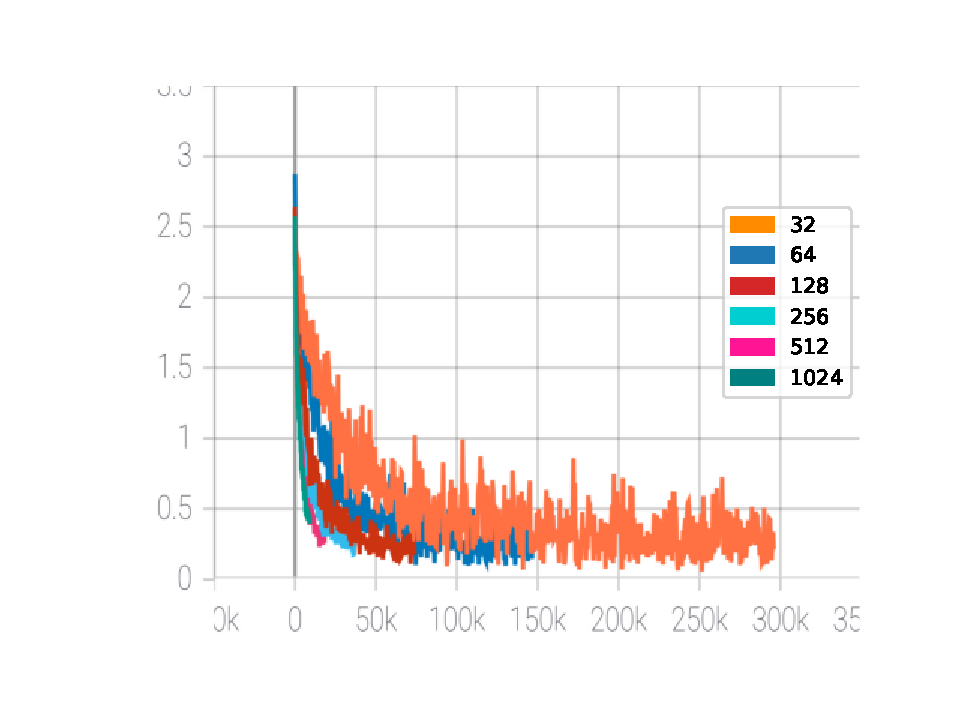
\includegraphics[width=0.45\textwidth]{byol-exp1/train_supervised_loss-no-smooth}%
        \label{fig:train:supervised:loss:nosmooth}%
        }%
    \hfill%
    \subfloat[Not smoothed top 1 accuracy ]{%
        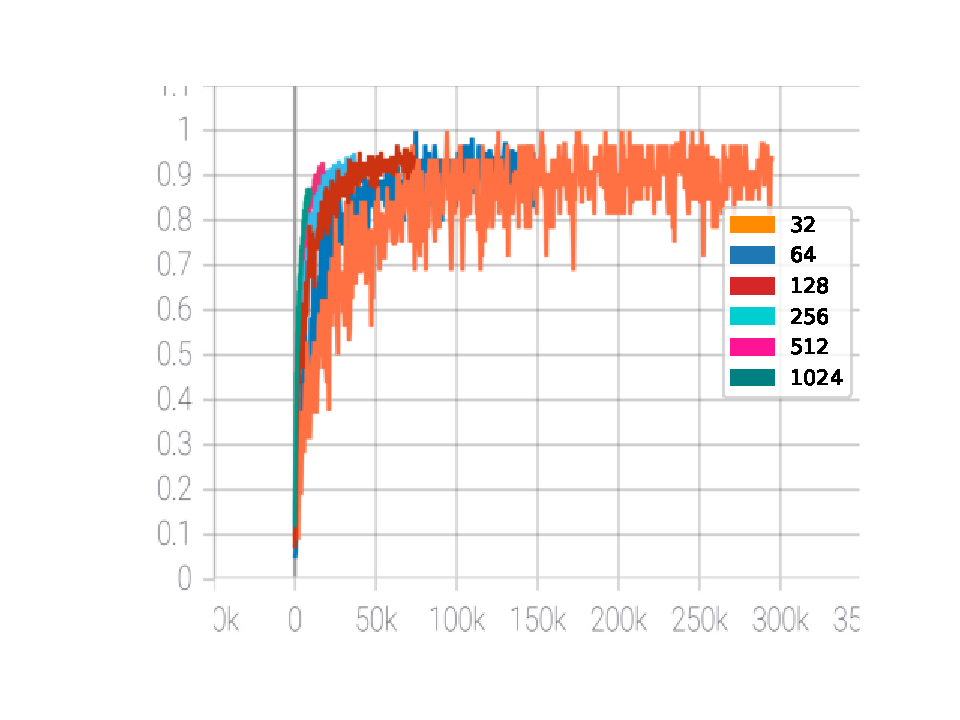
\includegraphics[width=0.45\textwidth]{byol-exp1/train_top_1_acc-no-smooth}%
        \label{fig:train:supervised:loss:nosmooth}%

        }%
        \caption{Examples of not smoothed charts in BYOL's experiments. }
        \label{fig:byol:not:smoothed}
\end{figure}

\subsection{Pre-sets on data augmentation and implementation possible improvements}
\label{byol:preset}

Data augmentation hyperparameters are not finetuned in this framework for a few reasons, including the long execution times. Despite this, since the importance of data augmentation has been recalled many times, we will explain the choice of hyperparameters that are pre-fixed in the implementation that we have chosen to run our experiments.

The first augmented view is applied the following transformations:
\begin{enumerate}
\item \emph{Random Flip}, selecting a random amount of images of the batch used and randomly flipping them.
\item \emph{Color Transformation}. This transformation is set to be applied with a probability of $1$, i.e., to always be applied. It adjusts the brightness, contrast and saturation of the image. It also has a probability of $0.8$ to apply color jitter and $0.2$ of transforming to grayscale. All this operations are shuffled to be applied in a random order.

\item \emph{Gaussian blur}. This transformation is also applied always to the image, using a $kernel\_size = \frac{\text{image size}}{\text{blur\_divider}}$, where we know that the image size is $32$ and \lstinline{blur_divider} is pre-fixed to $10$. Also, the standard deviations are in the range $[0.1,2]$.
\end{enumerate}

The second view follows the same process for the augmentations, but it is also sometimes (with probability $0.2$) applied a \emph{solarization}. This technique consists of reversing the tone of the whole or part of the image.


The original repository provides with the steps that can be followed to change the pre-sets of their code. However, we want to remark that the implementation could be generalized in some ways:
\begin{enumerate}
\item Firstly, this implementation has the hyperparameters for the data augmentation process are fixed, as we have just mentioned. This could be improved by adding more FLAGS or parameters to the \lstinline{main_loop.py} script. This would not be a huge cost for the implementation and would lead to a wider range of experimentation possibilities.

\item Along with the first change, the same could be done with not only the ResNet architecture, but also with the used dataset.
\end{enumerate}

This all can be changed manually to be able to run any experiment by modifying the source configurations provided. We also could have coded this generalization ourselves, but it was decided to focus on the experiments mentioned at the beginning of this section.

\subsection{First experiment: batch size influence}
\label{experiments:byol:first}

As we have stated, we would like to see how the batch size influences the representations obtained with this framework.  Beforehand, and recalling that the loss we use in this framework is written as follows
\[
\mathcal L_{\theta,\upxi} = \norm{\overline{q_\theta}(z_\theta) - \overline{z_\upxi'}}_2^2\quad , 
\]
we observe that, in contrast to SimCLR where the loss function compared $2N$ elements, there should be no correlation between the batch size and the loss function since only two elements are used to compute the loss. 

In this first experiment, we will fix ResNet18 as the encoder architecture, and will use the following values for the batch size parameter:
\[
\text{batch\_size} = \{32,64,128,256,512,1024\}    
\]
More values can not be tested since, if we try to use the following power of two, the execution fails indicating that the memory of the GPU cannot allocate the whole batch. Recall that for the experiment we also use the hyperparameters presented in Subsection \ref{byol:preset}.

If we run the experiments, we obtain the results that we fully present in Table \ref{table:byol:gridsearch:1}. 
\begin{table}[H]
    \resizebox{\columnwidth}{!}{
    \begin{tabular}{rrrrr}
    batch\_size & regularization\_loss & label\_top\_1\_accuracy & label\_top\_5\_accuracy & global\_step    \\ \hline
    32          & 0.723                & 0.875                   & 1                       & 295900          \\
    \textbf{64} & \textbf{0.381}       & \textbf{0.968}          & \textbf{1}              & \textbf{148000} \\
    128         & 0.436                & 0.929                   & 0.976                   & 739800          \\
    256         & 0.453                & 0.929                   & 0.996                   & 369900          \\
    512         & 0.520                & 0.916                   & 0.994                   & 184900          \\
    1024        & 0.752                & 0.852                   & 0.983                   & 924700         
    \end{tabular}
    }
    \caption{All results for BYOL's experiment on the influence of batch size.}
    \label{table:byol:gridsearch:1}
    \end{table}

We remark in the following table the two most important models obtained:

\begin{table}[H]
    \resizebox{\columnwidth}{!}{
    \begin{tabular}{rrrrr}
    batch\_size & regularization\_loss & label\_top\_1\_accuracy & label\_top\_5\_accuracy & global\_step    \\ \hline
    32          & 0.723                & 0.875                   & 1                       & 295900          \\
    \textbf{64} & \textbf{0.381}       & \textbf{0.968}          & \textbf{1}              & \textbf{148000} \\       
    \end{tabular}
    }
    \caption{Most important results for BYOL's experiment on the influence of batch size.}
    \label{table:byol:gridsearch:1}
    \end{table}

The models shown in Table \ref{table:byol:gridsearch:1} are the ones that obtain the highest value in top 1 accuracy score, which will be using to select the best model found. As we can see, in this case the \emph{best} models are the ones that use the smallest batch sizes, reaffirming the theory that batch size does not matter in this framework as much as it did in SimCLR.

\begin{figure}[htp] 
    \centering
    \subfloat[Representation loss in train]{%
        \includegraphics[width=0.45\textwidth]{byol-exp1/train_repr_loss}%
        \label{fig:repr:loss:exp1}%
        }%
    \hfill%
    \subfloat[Supervised loss in train]{%
        \includegraphics[width=0.45\textwidth]{byol-exp1/train_supervised_loss}%
        \label{fig:byol:supervised:loss:exp1}%

        }%
        \caption{Charts on the losses during train in the first experiment with BYOL framework. On axis $x$ we have the number of steps and on $y$ axis the value of the loss.}
        \label{fig:byol:exp1:both:losses}
\end{figure}

\begin{figure}[H]
\centering
\includegraphics[width=0.55\textwidth]{byol-exp1/train_total_loss}%
\caption{Total loss of all the models for the first experiment in BYOL. The axis are the same of the ones in Figure \ref{fig:byol:exp1:both:losses}. }
\label{fig:byol:total:loss:exp1}%
\end{figure}

As we can see in Figure \ref{fig:byol:total:loss:exp1}, the total loss (computed as the sum of both representation and supervised losses), achieves much lower values compared to SimCLR values: all of them are in the range $[0.7,1.4]$. This causes higher top 1 accuracy in classification. This is not surprising since this dataset is much smaller in terms of number of examples, so the model has facilities to learn from all the examples and possibly produce overfitting in the dataset.

Figures \ref{fig:repr:loss:exp1} and \ref{fig:byol:supervised:loss:exp1} show that the models with lower batch sizes flatten the curve more than the ones with lower values on this parameter. If we combine this information with the fact that the models with smaller batch size perform better in classification, we can state that the number of steps is relevant for an experiment like this, and more epochs should be given to the models with bigger batch sizes in order to let them train for a similar number of steps and verify if the models with smaller batch size still achieve better results in the downstream task than the ones with bigger batch size.


\subsection{Second experiment: ResNet depth influence}
\label{byol:second:experiment}

In the original paper, it is reported that BYOL benefits from larger encoder architectures as it happens in SimCLR. We want to experiment using the same architecture that we used in the last experiment with SimCLR, ResNet50, and test if we achieve better performance on the linear evaluation when we go deeper in the encoder architecture.

To be able to do this, we modify the \lstinline{configs/byol.py} script , changing the following variable to \lstinline{encoder_class='ResNet50'}. We run the main loop again and save the results using tensorboard records. All the results obtained are recorded in Table \ref{table:byol:gridsearch:2}.

\begin{table}[H]
    \resizebox{\columnwidth}{!}{
    \begin{tabular}{rrrrr}
    batch\_size  & regularization\_loss & label\_top\_1\_accuracy & label\_top\_5\_accuracy & global\_step    \\ \hline
    32           & 0.564                & 0.937                   & 0.9688                  & 295900          \\
    64           & 0.484                & 0.953                   & 1                       & 148000          \\
    \textbf{128} & \textbf{0.2747}      & \textbf{1}              & \textbf{1}              & \textbf{739800} \\
    256          & 0.276                & 0.968                   & 1                       & 369900         
    \end{tabular}
    }
    \caption{All results for BYOL's experiment on the influence of the encoder architecture.}
\label{table:byol:gridsearch:2}
    \end{table}

\begin{table}[H]
    \resizebox{\columnwidth}{!}{
    \begin{tabular}{rrrrrr}
    ResNet    & batch\_size  & regularization\_loss & label\_top\_1\_accuracy & label\_top\_5\_accuracy & global\_step    \\ \hline
    18          & 32           & 0.723                & 0.875                   & 1                       & 295900          \\
              & 64           & 0.381                & 0.968                   & 1                       & 148000          \\
    \textbf{50} & \textbf{128} & \textbf{0.2747}      & \textbf{1}              & \textbf{1}              & \textbf{739800} \\
              & 256          & 0.276                & 0.968                   & 1                       & 369900         
    \end{tabular}
    }
    \caption{Results of the best models in both first and second experiments with BYOL.}
    \label{table:byol:exp2:comparison}
    \end{table}

In Table \ref{table:byol:exp2:comparison} we report the best two models of each of the experiments performed with BYOL. As we can see, the model that obtains the highest top 1 accuracy is the one that uses ResNet50 as the encoder, that is, the one with deeper encoder architecture. 

We also have to remark that the best model achieves perfect accuracy on the classification task, which is really surprising. The representations that the model is creating for the Imagenette dataset are very accurate, so the linear head can classify all the elements in the test set correctly. Also, as we can see, all the models obtain $100\%$ top 5 accuracy, which means that even if the prediction that the linear head does is not correct, it is always close to be correct, so this informs us that our models advance towards learning representations that contain a lot of information about the original input.


\begin{figure}[htp] 
    \centering
    \subfloat[Representation loss in train]{%
        \includegraphics[width=0.45\textwidth]{byol-exp2/train_repr_loss}%
        \label{fig:repr:loss:exp2}%
        }%
    \hfill%
    \subfloat[Supervised loss in train]{%
        \includegraphics[width=0.45\textwidth]{byol-exp2/train_supervised_loss}%
        \label{fig:byol:supervised:loss:exp2}%

        }%
        \caption{Charts on the losses during train in the second experiment with BYOL framework. On axis $x$ we have the number of steps and on $y$ axis the value of the loss.}
        \label{fig:byol:exp2:both:losses}
\end{figure}

\begin{figure}[H]
\centering
\includegraphics[width=0.55\textwidth]{byol-exp2/train_total_loss}%
\caption{Total loss of the models that we are comparing in the second experiment done using BYOL. The axis are the same of the ones in Figure \ref{fig:byol:exp2:both:losses}. }
\label{fig:byol:total:loss:exp2}%
\end{figure}

Observing Figure \ref{fig:repr:loss:exp2}, we can see that the selected as best models reach really low values on the representation loss. This is consistent with the results that we later obtain using these representations for the classification task with the linear head. The model with the biggest batch size performs the fewest number of steps, and it does not achieve to completely flatten the loss curve. However, this is not bad news, since it indicates that this model can still improve in the representation learning task and, therefore, improve the final accuracy score on the classification task.

In Figure \ref{fig:byol:supervised:loss:exp2} we can see that, in the supervised part, the improvement can come from any of the models, since none of them completely flattens the loss curve in the amount of steps that we have set for them. Adding the two losses we obtain the total loss represented in Figure \ref{fig:byol:total:loss:exp2}. If we remember the first experiment, the range for the total loss was $[0.7,1.4]$, in this case the total loss values are reduced to the range $[0.4,0.7]$ which indicates lower losses in general. This is also consistent with the better accuracy scores in the linear evaluation.


\subsection{Evaluating ResNet50 models to test performance}

As we have mentioned before, the already presented results were obtained in the train set, which has no value in the machine learning field. Our last step in this experimentation was to test the models obtained in a \emph{test} set. The original code provided with a parameter option that allowed us to do this.

\subsection{Conclusions about BYOL}

With the two experiments that we have done using BYOL, we can conclude the following:
\begin{itemize}
\item Unlike SimCLR, \lstinline{batch_size} is not a key hyperparameter for the performance of the framework. In fact, one of the smallest batch size values tested obtained the best result in the first experiment.

\item As in SimCLR, the encoder depth influences the final results on the classification task and, therefore, we can assume that influences the quality of the representations for any downstream task performed.


\item The accuracies that this framework obtains are quite higher compared to SimCLR's scores. Recall that both models were pretrained from zero, but trained in different datasets. However, the difference between the datasets should not be a discriminator, since both of them have similar properties (in terms of number of classes and separability of the classes) and the main difference is the number of examples.


\end{itemize}

Recall that we achieved $100\%$ top 1 accuracy in \emph{train} in one of our executions. This may indicate that we are overfitting our train set. However, when we evaluated the models in the train set and although the final accuracy was still very high, we did not classify the whole test set correctly. We obtained the following model:


\begin{table}[H]
  \resizebox{\columnwidth}{!}{
    \begin{tabular}{rrrrr}
      batch\_size  & loss & top\_1\_accuracy & top\_5\_accuracy & steps    \\ \hline
      
      \textbf{64} & \textbf{0.381}       & \textbf{0.9240764}          & \textbf{1}              & \textbf{148000} \\       
    \end{tabular}
    }
    \caption{Conclusion of the experiments with BYOL.}
    \label{table:byol:conclusions}
    \end{table}
